% 仅子章节内容，宏包统一在主文件导入
\section{触发器基础题}

% 题 5.1
\subsection{题 5.1：与非门 SR 锁存器波形}

题目：画出图中由与非门组成的 SR 锁存器输出端 $Q$、$\overline{Q}$ 的电压波形，输入端 $\overline{S_D}$、$\overline{R_D}$ 的电压波形如图中所示。

\begin{center}
    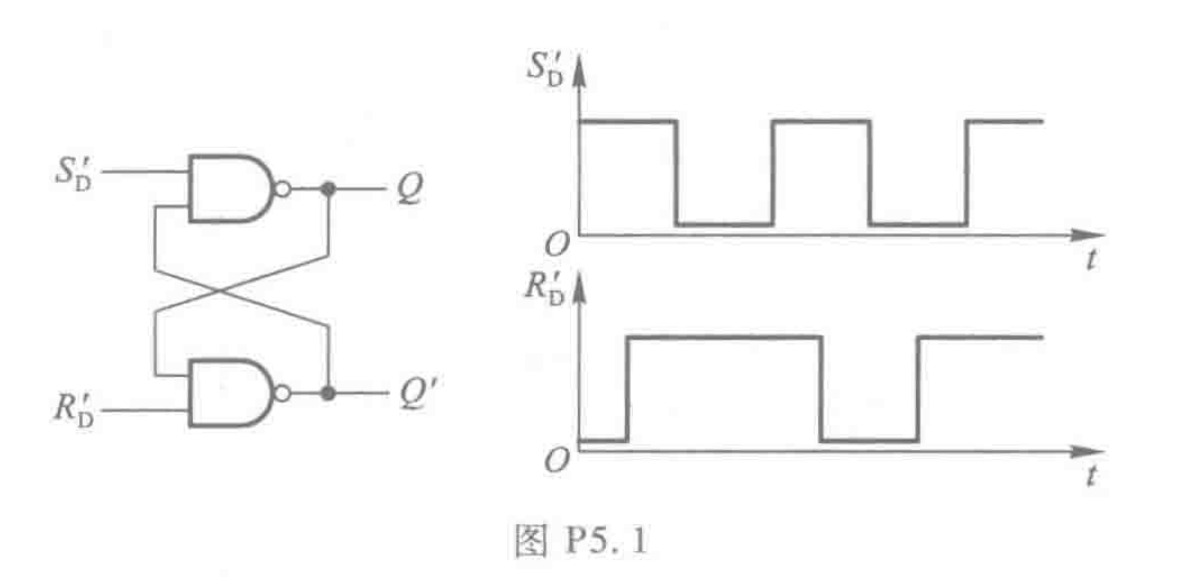
\includegraphics[width=0.45\textwidth]{5.1.png}
\end{center}

\textbf{解答：}

与非门构成的 SR 锁存器为低电平有效，特性表如下：

\begin{center}
\begin{tabular}{cccc}
\toprule
$\overline{S_D}$ & $\overline{R_D}$ & $Q$ & 功能 \\
\midrule
1 & 1 & 保持 & 锁存 \\
1 & 0 & 0 & 置 0（复位）\\
0 & 1 & 1 & 置 1（置位）\\
0 & 0 & 不定 & 禁止态 \\
\bottomrule
\end{tabular}
\end{center}

设初始状态 $Q=0$，根据输入波形逐段分析：
\begin{enumerate}
    \item $\overline{S_D}=1,\ \overline{R_D}=0$：置 0，$Q=0$
    \item $\overline{S_D}=1,\ \overline{R_D}=1$：保持，$Q=0$
    \item $\overline{S_D}=0,\ \overline{R_D}=1$：置 1，$Q=1$
    \item $\overline{S_D}=1,\ \overline{R_D}=1$：保持，$Q=1$
    \item $\overline{S_D}=0,\ \overline{R_D}=0$：禁止态，$Q$ 与 $\overline{Q}$ 均为 1
    \item $\overline{S_D}=1,\ \overline{R_D}=1$：恢复保持，状态取决于优先解除禁止的输入端
\end{enumerate}

% 手绘标准时序波形图
\begin{center}
\begin{tikzpicture}[scale=0.7,line width=0.7pt]
% 纵坐标标注
\foreach \y/\lab in {6/$\overline{S_D}$,4/$\overline{R_D}$,2/$Q$,0/$\overline{Q}$}
    \node[left] at (-0.5,\y) {\lab};
% 时间刻度
\foreach \x in {0,1,2,3,4,5,6,7,8}
    \draw (\x,7) -- (\x,-1);

% 绘制SD非波形
\draw (0,6) -- (2,6) -- (2,5) -- (3,5) -- (3,6) -- (5,6) -- (5,5) -- (6,5) -- (6,6) -- (8,6);
% 绘制RD非波形
\draw (0,5) -- (1,5) -- (1,4) -- (4,4) -- (4,5) -- (6,5) -- (6,4) -- (8,4);
% 绘制Q波形
\draw (0,2) -- (3,2) -- (3,3) -- (5,3) -- (6,3) -- (6,2.5) -- (8,2);
% 绘制Q非波形
\draw (0,3) -- (3,3) -- (3,2) -- (5,2) -- (6,2) -- (6,2.5) -- (8,3);

% 高低电平标注
\node[right] at (8.2,6) {高};
\node[right] at (8.2,5) {低};
\end{tikzpicture}
\end{center}

\textbf{结论：}
\begin{itemize}
    \item $\overline{S_D}$ 低电平置 1，$\overline{R_D}$ 低电平置 0，均为高电平时保持。
    \item 除禁止态外，$\overline{Q}$ 与 $Q$ 始终互补。
\end{itemize}

\vspace{1em}
\hrulefill
\vspace{1em}

% 题 5.2
\subsection{题 5.2：或非门 SR 锁存器波形}

题目：画出图中由或非门组成的 SR 锁存器输出端 $Q$、$\overline{Q}$ 的电压波形，输入端 $S_D$、$R_D$ 的电压波形如图中所示。

\begin{center}
    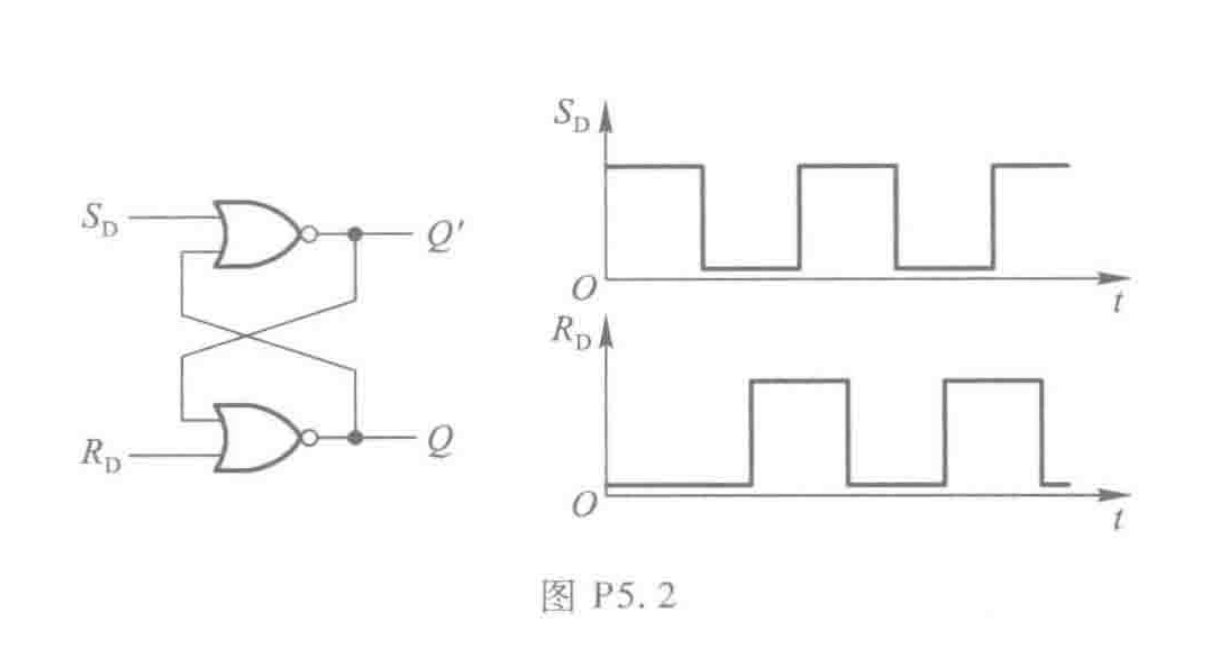
\includegraphics[width=0.45\textwidth]{5.2.png}
\end{center}

\textbf{解答：}

或非门构成的 SR 锁存器为高电平有效，特性表如下：

\begin{center}
\begin{tabular}{cccc}
\toprule
$S_D$ & $R_D$ & $Q$ & 功能 \\
\midrule
0 & 0 & 保持 & 锁存 \\
0 & 1 & 0 & 置 0（复位）\\
1 & 0 & 1 & 置 1（置位）\\
1 & 1 & 不定 & 禁止态 \\
\bottomrule
\end{tabular}
\end{center}

设初始状态 $Q=0$，逐段分析：
\begin{enumerate}
    \item $S_D=1,\ R_D=0$：置 1，$Q=1$
    \item $S_D=0,\ R_D=0$：保持，$Q=1$
    \item $S_D=0,\ R_D=1$：置 0，$Q=0$
    \item $S_D=1,\ R_D=0$：置 1，$Q=1$
    \item $S_D=0,\ R_D=1$：置 0，$Q=0$
\end{enumerate}

% 时序波形图
\begin{center}
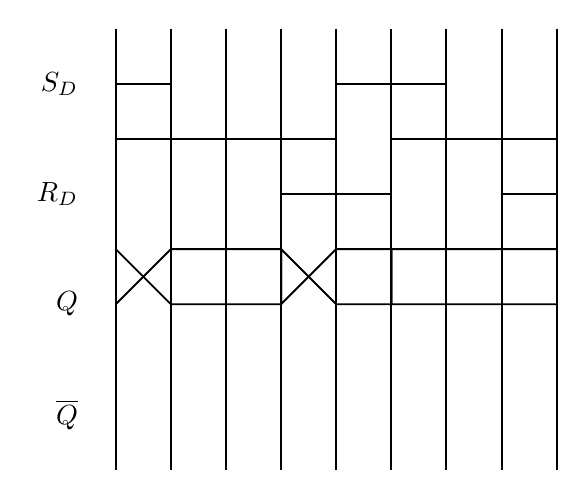
\begin{tikzpicture}[scale=0.7,line width=0.7pt]
\foreach \y/\lab in {6/$S_D$,4/$R_D$,2/$Q$,0/$\overline{Q}$}
    \node[left] at (-0.5,\y) {\lab};
\foreach \x in {0,1,2,3,4,5,6,7,8}
    \draw (\x,7) -- (\x,-1);

\draw (0,6) -- (1,6) -- (1,5) -- (4,5) -- (4,6) -- (6,6) -- (6,5) -- (8,5);
\draw (0,5) -- (3,5) -- (3,4) -- (5,4) -- (5,5) -- (7,5) -- (7,4) -- (8,4);
\draw (0,2) -- (1,3) -- (3,3) -- (3,2) -- (4,3) -- (5,3) -- (5,2) -- (8,2);
\draw (0,3) -- (1,2) -- (3,2) -- (3,3) -- (4,2) -- (5,2) -- (5,3) -- (8,3);
\end{tikzpicture}
\end{center}

\textbf{结论：}
\begin{itemize}
    \item $S_D=1$ 置 1，$R_D=1$ 置 0，均为 0 时保持。
    \item 除禁止态外，$\overline{Q}$ 与 $Q$ 互补。
\end{itemize}

\vspace{1em}
\hrulefill
\vspace{1em}

% 题 5.9
\subsection{题 5.9：边沿触发 JK 触发器波形}

题目：已知边沿触发 JK 触发器各输入端电压波形如图所示，画出输出 $Q$、$\overline{Q}$ 的波形。

\begin{center}
    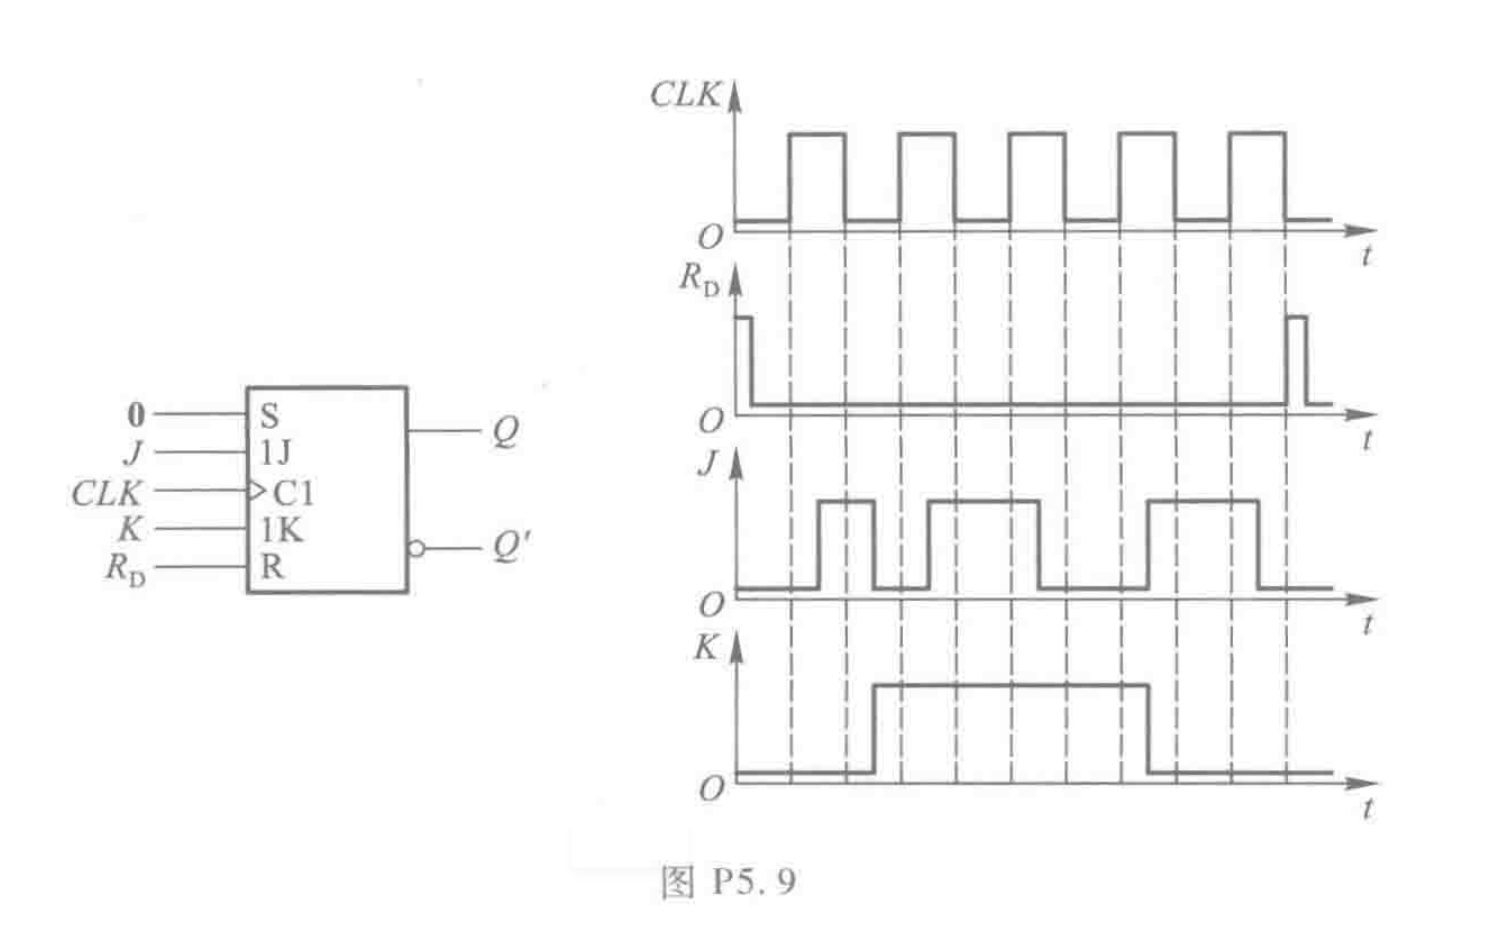
\includegraphics[width=0.5\textwidth]{5.9.png}
\end{center}

\textbf{解答：}

该触发器为 \textbf{下降沿触发} 的 JK 触发器，异步复位端 $\overline{R_D}$ 低电平有效，优先级最高。

特性方程：
\[
Q^{n+1} = J\overline{Q^n} + \overline{K}Q^n
\]

设初始状态 $Q=0$，逐周期分析：
\begin{enumerate}
    \item $\overline{R_D}=0$：强制置 0，$Q=0$
    \item 第 1 个时钟下降沿：$J=0,K=0$，保持 $Q=0$
    \item 第 2 个时钟下降沿：$J=1,K=1$，翻转，$Q=1$
    \item 第 3 个时钟下降沿：$J=1,K=1$，翻转，$Q=0$
    \item 第 4 个时钟下降沿：$J=0,K=1$，置 0，$Q=0$
    \item 第 5 个时钟下降沿：$J=1,K=0$，置 1，$Q=1$
    \item 最后 $\overline{R_D}=0$：强制置 0，$Q=0$
\end{enumerate}

% JK触发器完整时序图
\begin{center}
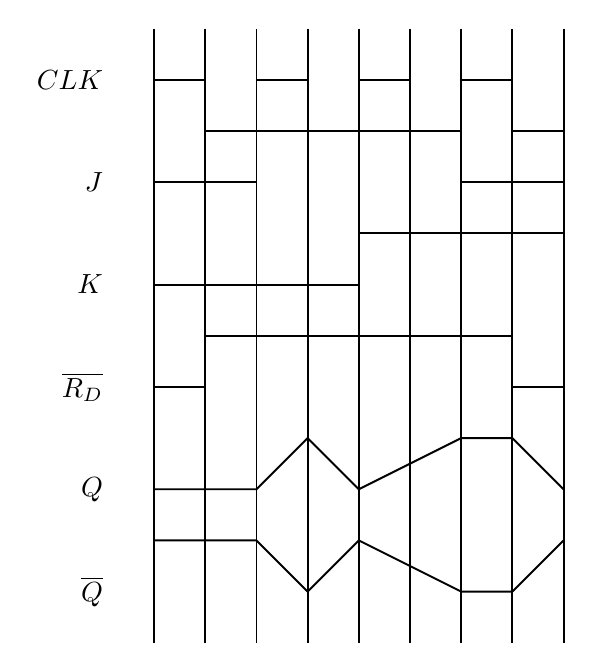
\begin{tikzpicture}[scale=0.65,line width=0.7pt]
\foreach \y/\lab in {8/$CLK$,6/$J$,4/$K$,2/$\overline{R_D}$,0/$Q$,-2/$\overline{Q}$}
    \node[left] at (-0.8,\y) {\lab};
\foreach \x in {0,1,2,3,4,5,6,7,8}
    \draw (\x,9) -- (\x,-3);

% 时钟波形
\draw (0,7)--(0,8)--(1,8)--(1,7)--(2,7)--(2,8)--(3,8)--(3,7)
      --(4,7)--(4,8)--(5,8)--(5,7)--(6,7)--(6,8)--(7,8)--(7,7)--(8,7);
% J波形
\draw (0,6)--(2,6)--(2,7)--(6,7)--(6,6)--(8,6);
% K波形
\draw (0,4)--(4,4)--(4,5)--(8,5);
% 异步复位
\draw (0,2)--(1,2)--(1,3)--(7,3)--(7,2)--(8,2);
% Q输出
\draw (0,0)--(2,0)--(3,1)--(4,0)--(6,1)--(7,1)--(8,0);
% Q非输出
\draw (0,-1)--(2,-1)--(3,-2)--(4,-1)--(6,-2)--(7,-2)--(8,-1);
\end{tikzpicture}
\end{center}

\textbf{结论：}
\begin{itemize}
    \item 状态仅在时钟下降沿更新。
    \item 异步复位 $\overline{R_D}=0$ 可随时强制置 0，与时钟无关。
    \item $\overline{Q}$ 始终与 $Q$ 电平互补。
\end{itemize}